\documentclass[12pt]{article}

\usepackage{../thesis}

\usepackage{tikz} 
\usepackage{pgfplots} % drawing plots right here in this file!
\pgfplotsset{compat=1.9} % latest stable release
\usepgfplotslibrary{statistics}

\pgfplotsset{
  every axis/.append style={
    scale only axis,
    width=2.4in,
  },
  /tikz/every picture/.append style={
    baseline
  }
}

\begin{document}

\pagestyle{empty}

  \begin{tikzpicture}[trim axis left]
	\begin{semilogyaxis}[xmin=-2,xmax=105,
        width=5.7in, height=2.5in,
		title={Servo Rolloff},
		xlabel={Servo gain $I$}, ylabel={$\tau_{servo}$ (s)},
        boxplot/draw direction=y,]
        \addplot[boxplot prepared={draw position=1,box extend=3,lower whisker=2.527756e-03,lower quartile=3.926641e-03,median=8.583072e-03,upper quartile=2.097231e-02,upper whisker=8.373186e-02,},] coordinates {};
        \addplot[boxplot prepared={draw position=5,box extend=3,lower whisker=6.960332e-04,lower quartile=8.624233e-04,median=1.183870e-03,upper quartile=2.002728e-03,upper whisker=2.759733e-03,},] coordinates {};
        \addplot[boxplot prepared={draw position=10,box extend=3,lower whisker=3.261403e-04,lower quartile=3.943302e-04,median=5.551368e-04,upper quartile=9.875646e-04,upper whisker=1.418181e-03,},] coordinates {};
        \addplot[boxplot prepared={draw position=20,box extend=3,lower whisker=1.397812e-04,lower quartile=1.776975e-04,median=2.437888e-04,upper quartile=4.560549e-04,upper whisker=6.031656e-04,},] coordinates {};
        \addplot[boxplot prepared={draw position=30,box extend=3,lower whisker=7.250511e-05,lower quartile=1.017245e-04,median=1.436788e-04,upper quartile=3.071162e-04,upper whisker=3.903013e-04,},] coordinates {};
        \addplot[boxplot prepared={draw position=40,box extend=3,lower whisker=3.912787e-05,lower quartile=6.020131e-05,median=9.202824e-05,upper quartile=2.075595e-04,upper whisker=2.666014e-04,},] coordinates {};
        \addplot[boxplot prepared={draw position=50,box extend=3,lower whisker=1.897719e-05,lower quartile=3.445664e-05,median=6.100964e-05,upper quartile=1.539548e-04,upper whisker=2.185083e-04,},] coordinates {};
        \addplot[boxplot prepared={draw position=60,box extend=3,lower whisker=8.880600e-11,lower quartile=1.652902e-05,median=4.002564e-05,upper quartile=1.229701e-04,upper whisker=1.827573e-04,},] coordinates {};
        \addplot[boxplot prepared={draw position=70,box extend=3,lower whisker=1.755270e-11,lower quartile=9.542594e-10,median=2.435035e-05,upper quartile=9.756506e-05,upper whisker=1.397686e-04,},] coordinates {};
        \addplot[boxplot prepared={draw position=80,box extend=3,lower whisker=2.593788e-12,lower quartile=2.047951e-10,median=1.087006e-05,upper quartile=7.457268e-05,upper whisker=1.102265e-04,},] coordinates {};
        \addplot[boxplot prepared={draw position=90,box extend=3,lower whisker=4.877739e-13,lower quartile=9.832435e-11,median=1.889502e-09,upper quartile=6.005101e-05,upper whisker=9.565394e-05,},] coordinates {};
        \addplot[boxplot prepared={draw position=100,box extend=3,lower whisker=5.761899e-13,lower quartile=9.181211e-11,median=1.220353e-09,upper quartile=5.130300e-05,upper whisker=1.918065e-04,},] coordinates {};
	\end{semilogyaxis}
  \end{tikzpicture}

\begin{tabular}{rr}

  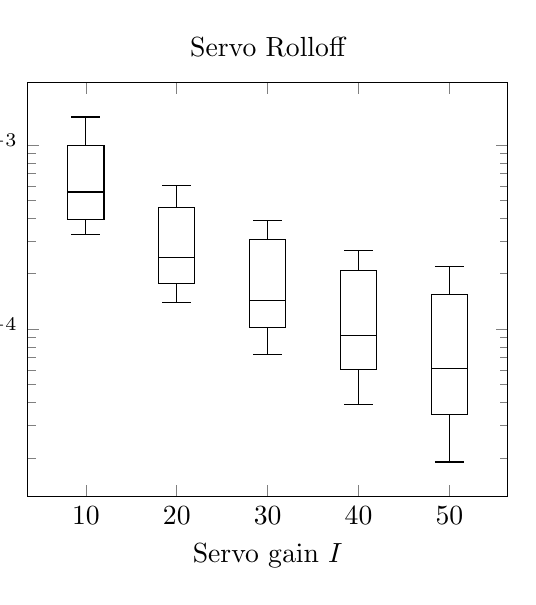
\begin{tikzpicture}[trim axis left]
	\begin{semilogyaxis}[%ymin=0,%xmin=950,xmax=1250,
		title={Servo Rolloff},
		xlabel={Servo gain $I$}, ylabel={$\tau_{servo}$ (s)},
        boxplot/draw direction=y,]
        \addplot[boxplot prepared={draw position=10,box extend=4,lower whisker=3.261403e-04,lower quartile=3.943302e-04,median=5.551368e-04,upper quartile=9.875646e-04,upper whisker=1.418181e-03,},] coordinates {};
        \addplot[boxplot prepared={draw position=20,box extend=4,lower whisker=1.397812e-04,lower quartile=1.776975e-04,median=2.437888e-04,upper quartile=4.560549e-04,upper whisker=6.031656e-04,},] coordinates {};
        \addplot[boxplot prepared={draw position=30,box extend=4,lower whisker=7.250511e-05,lower quartile=1.017245e-04,median=1.436788e-04,upper quartile=3.071162e-04,upper whisker=3.903013e-04,},] coordinates {};
        \addplot[boxplot prepared={draw position=40,box extend=4,lower whisker=3.912787e-05,lower quartile=6.020131e-05,median=9.202824e-05,upper quartile=2.075595e-04,upper whisker=2.666014e-04,},] coordinates {};
        \addplot[boxplot prepared={draw position=50,box extend=4,lower whisker=1.897719e-05,lower quartile=3.445664e-05,median=6.100964e-05,upper quartile=1.539548e-04,upper whisker=2.185083e-04,},] coordinates {};
	\end{semilogyaxis}
  \end{tikzpicture}

  &

  \begin{tikzpicture}[trim axis right]
	\begin{axis}[ymin=0,%xmin=950,xmax=1250,
		title={\SQUID\ Noise},
		xlabel={Servo gain $I$}, ylabel={Median Noise (\Inoise{})},
        ]
	  \addplot+[only marks] table[x=gain,y=noise]{../data/ch8-servo-noise-vs-gain.dat};
	  %\addplot+[only marks] table[x=gain,y=noise]{../data/ch8-servo-ds.dat};
	\end{axis}
  \end{tikzpicture}

  %% \begin{tikzpicture}[trim axis right]
  %%   \begin{semilogyaxis}[ymin=1e-11,ymax=1e-2,
  %%   	title={\SQUID\ Noise Rolloff ($I$ = 60)},
  %%   	xlabel={Readout Row}, ylabel={$\tau_{servo}$ (s)},
  %%       legend pos=north west]
  %%     \addplot+[only marks] table[x=R,y=tau60]{../data/ch8-servo-sc0.dat};
  %%     %\addlegendentry {Col 0}
  %%     \addplot+[only marks] table[x=R,y=tau60]{../data/ch8-servo-sc1.dat};
  %%     %\addlegendentry {Col 1}
  %%     \addplot+[only marks] table[x=R,y=tau60]{../data/ch8-servo-sc2.dat};
  %%     %\addlegendentry {Col 2}
  %%     \addplot+[only marks] table[x=R,y=tau60]{../data/ch8-servo-sc3.dat};
  %%     %\addlegendentry {Col 3}
  %%     \addplot+[only marks] table[x=R,y=tau60]{../data/ch8-servo-sc4.dat};
  %%     %\addlegendentry {Col 4}
  %%     \addplot+[only marks] table[x=R,y=tau60]{../data/ch8-servo-sc5.dat};
  %%     %\addlegendentry {Col 5}
  %%     \addplot+[only marks] table[x=R,y=tau60]{../data/ch8-servo-sc6.dat};
  %%     %\addlegendentry {Col 6}
  %%     \addplot+[only marks] table[x=R,y=tau60]{../data/ch8-servo-sc7.dat};
  %%     %\addlegendentry {Col 7}
  %%   \end{semilogyaxis}
  %% \end{tikzpicture}

  \\
\end{tabular}
\end{document}
